\documentclass[a4paper,12pt]{scrartcl}
\usepackage[utf8]{inputenc}
\usepackage[T1]{fontenc}
\usepackage[french]{babel}
\usepackage{graphics}
\usepackage{graphicx}
\usepackage{enumitem}
\usepackage[margin=2cm]{geometry}
\usepackage{amsmath}
\usepackage{amssymb}
\usepackage{hyperref}
\usepackage{float}
\usepackage{empheq}
\usepackage[table,xcdraw]{xcolor}
\usepackage{lmodern,textcomp}
\usepackage{tcolorbox}
\usepackage{karnaugh-map}



% Change itemize dash by bullet

\renewcommand{\labelitemi}{$\bullet$}

% Bulma CSS framework color, see : https://bulma.io/documentation/overview/colors/

\definecolor{primary}{HTML}{00d1b2}
\definecolor{link}{HTML}{3273dc}
\definecolor{info}{HTML}{209cee}
\definecolor{success}{HTML}{48c774}
\definecolor{warning}{HTML}{ffdd57}
\definecolor{danger}{HTML}{ff3860}

% Command for easier color management in tcolorbox

\newenvironment{titletbox}[2] % 1 = title, 2 = color
  {\tcolorbox[noparskip,colback=#2!5!white,colframe=#2!75!black,arc=1mm,title=#1,halign title = center]}
  {\endtcolorbox}

\newenvironment{tbox}[1] % 1 = color
  {\tcolorbox[noparskip,colback=#1!5!white,colframe=#1!75!black,arc=1mm]}
  {\endtcolorbox}



% hyperlinks setup 

\hypersetup{
  colorlinks=true,
  linkcolor=cyan,
  filecolor=magenta,      
  urlcolor=blue,
  pdfpagemode=FullScreen,
}



\begin{document}

    \begin{titlepage}

    \newcommand{\HRule}{\rule{\linewidth}{0.5mm}} 							% horizontal line and its thickness
    \center 
     
    % University
    
\includegraphics[width=\textwidth]{../pictures/UCLouvain-EPL.png}\\[1cm]
    
    % Document info
    \textsc{\large 
    LINFO1140 - Bases électroniques de l'informatique}\\[1cm] 										% Course Code
    \HRule \\[0.8cm]
    {\huge \bfseries Travail 6 - circuit CMOS}\\[0.7cm]								% Assignment
    \HRule \\[2cm]
    \large
    \emph{Auteur:}\\
    Nicolas Jeanmenne\\[1.5cm]
    \emph{Noma:}\\
    4874-19-00\\[1.5cm]
    \vfill													% Author info
    {\large 2021-2022}\\[5cm] 	% University logo
    
    \vfill
\end{titlepage}

    \section{Introduction}

    \subparagraph{}Le but de ce {\color{info}3\ieme{} travail} est d'implémenter un circuit contenant au moins une source de tension ainsi qu'une source de courant avec 
    5 résistances. Il s'agira ensuite de calculer les équivalents de Thévenin et Norton et enfin de simuler le circuit avec le logiciel \textit{LTspice}
    afin de démontrer l'exactitude des calculs.\\[1.5cm]
    
    \begin{titletbox}{À l'attention du correcteur / correctrice}{warning}
        N'hésitez pas à zoomer sur les schémas du circuit et autres images afin d'y voir plus clair.
    \end{titletbox}

\section{Schéma initial du circuit}

    \begin{figure}[H]
        \centering
        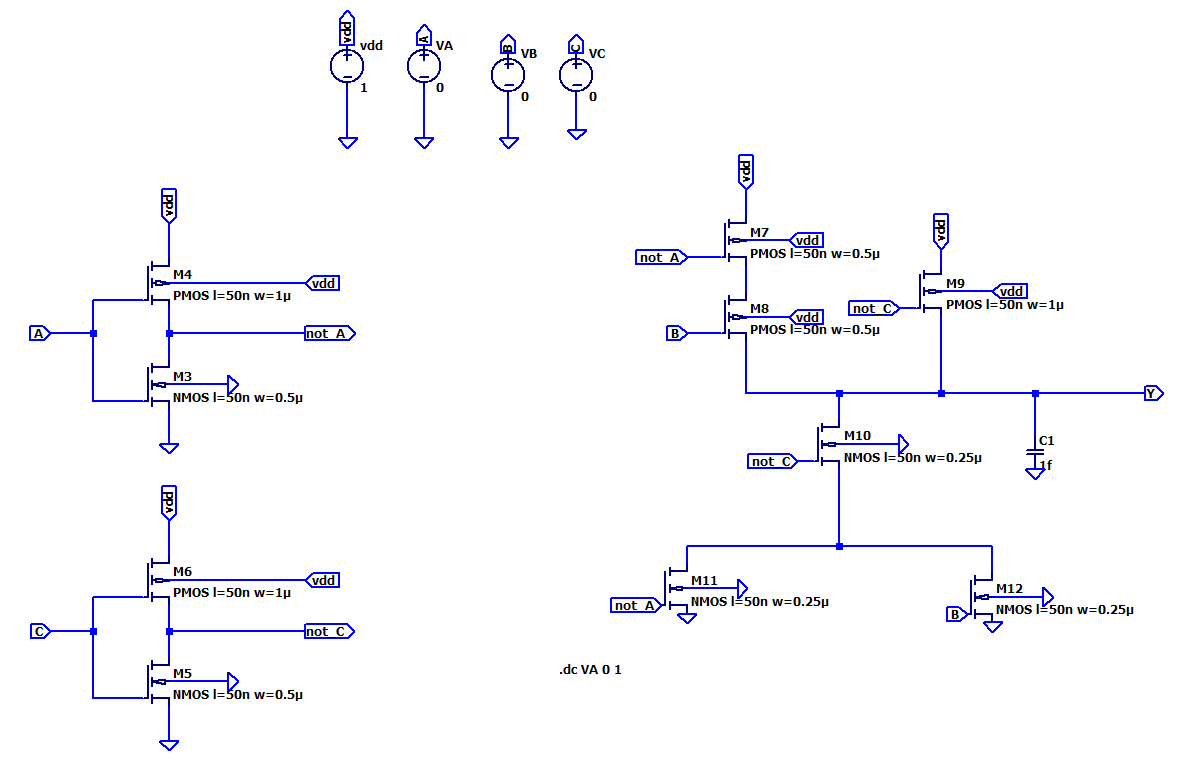
\includegraphics[scale=0.5]{../pictures/circuit.png} % Pas utiliser width=\textwidth pcq il prend la taille de \section{} comme ref
        \caption{Schéma du circuit}
    \end{figure}

    \begin{figure}[H]
        \centering
        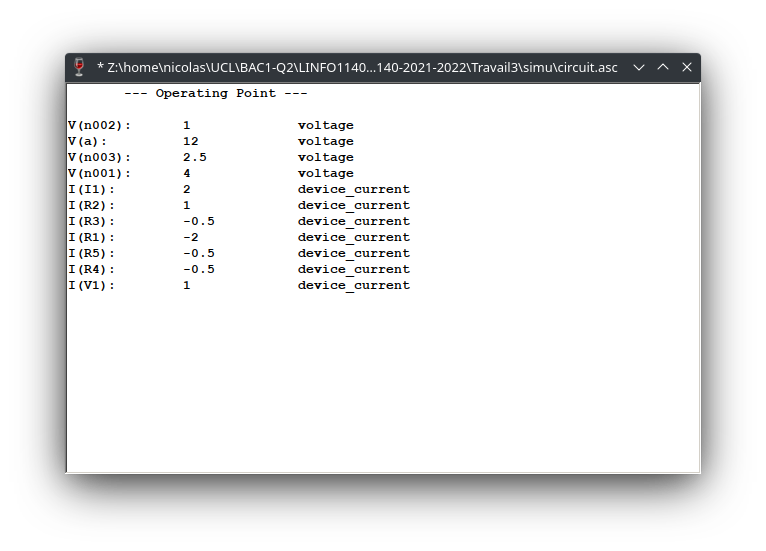
\includegraphics[scale=0.8]{../pictures/resultat.png} % Pas utiliser width=\textwidth pcq il prend la taille de \section{} comme ref
        \caption{Résultat du circuit}
    \end{figure}

\section{Calcul de la résistance équivalente}

    \subparagraph{}En premier lieu, il faut annuler les sources, comme elles ne sont pas commandées la source de courant devient un circuit ouvert et la source de tension un court-circuit.
    
        \begin{figure}[h!]
                \centering
                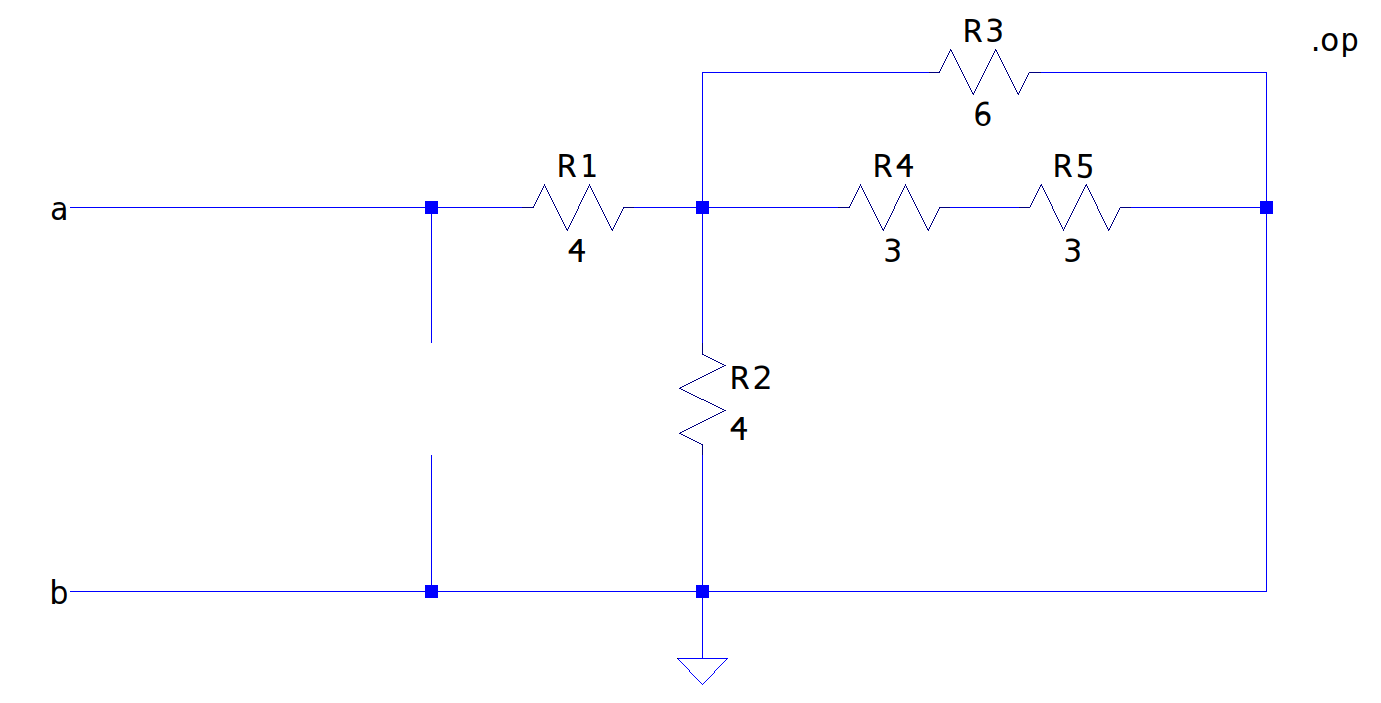
\includegraphics[width=\textwidth]{../pictures/cancel.png}
                \caption{Annulation des sources}
                \label{cancel}
            \end{figure}
            
    \subparagraph{} La résistance équivalente se calcule donc comme tel :
        
        \begin{align*}
            R_{eq} \; &= \; ((R_3 \; // \; (R_4 \; + \; R_5)) \; // \; R_2) \; + \; R_1 
        \end{align*}
        
        \begin{align*}
            R_4\;+\;R_5\;&=\;3\;+\;3 \\
            R_4\;+\;R_5\;&=\;6\;\Omega \\
        \end{align*}
        
        \begin{align*}
            R_3\;//\;(R_4 + R_5)\;&=\;\frac{6 \cdot 6}{6 + 6} \\
            R_3\;//\;(R_4 + R_5)\;&=\;\frac{36}{12} \\
            R_3\;//\;(R_4 + R_5)\;&=\;3\;\Omega
        \end{align*}
        
        \begin{align*}
            (R_3\;//\;(R_4 + R_5))\;//\;R_2)\;&=\;\frac{3 \cdot 4}{3 + 4} \\
            (R_3\;//\;(R_4 + R_5))\;//\;R_2)\;&=\;\frac{12}{7} \\
            (R_3\;//\;(R_4 + R_5))\;//\;R_2)\;&=\;1.714285714\;\Omega
        \end{align*}
        
        \begin{align*}
            R_{eq}\;&=\;\frac{12}{7} + R_1 \\
            R_{eq}\;&=\;\frac{12}{7} + 4 \\
        \end{align*}
        
        \begin{empheq}[box=\fbox]{equation*}
            R_{eq}\;=\;\frac{40}{7}\;(\approx\;5.714285714)\;\;\Omega
        \end{empheq}

\section{Calcul des équivalents}

    \subsection{Tension de Thévenin}
    
        \subparagraph{}D'abord je vais simplifier quelques résistances pour simplifier les calculs :
        
        \begin{figure}[H]
            \centering
            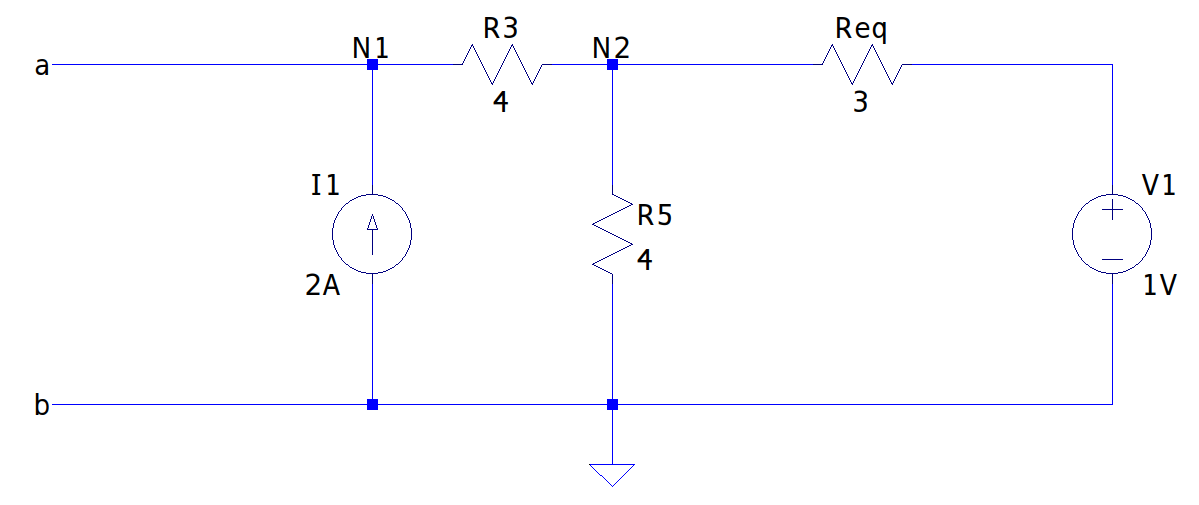
\includegraphics[width=\textwidth]{../pictures/simple.png}
            \caption{Circuit simplifié}
            \label{simple}
        \end{figure}
        
        \subparagraph{}Ensuite je vais utiliser la méthode des noeuds, vu que le ground symbol nous permet de dire que la tension à son noeud = 0V, nous savons que $V_{N_1}$ = $V_{Th}$. Enfin pour que les équations soient plus claires, on pose $V_{N_2}$ = $V_x$ :
        
            \begin{equation*}
            \left \{
               \begin{array}{r c l}
                  2\;&=\;\frac{V_{Th} - V_x}{4} \\
                  \frac{V_x}{4}\;&=\;\frac{V_{Th} - V_x}{4}\;+\;\frac{1 - V_x}{3}
               \end{array}
           \right .
        \end{equation*}
        
        \subparagraph{}En substituant, on trouve $V_x = 4$, on peut donc le remplacer dans la $2^{ème}$ équation :
        
            \begin{align*}
                \frac{4}{4}\;&=\;\frac{V_{Th}-4}{4} + \frac{1 - 4}{3} \\
                1\;&=\;\frac{V_{Th}-4}{4} + \frac{-3}{3} \\
                4\;&=\;V_{Th} - 4 -4 \\
                V_{Th}\;&=\;12\;V
            \end{align*}
            
            
    \subsection{Courant de Norton}
    
        \subparagraph{}Comme on a la résistance équivalente et la tension de Thévenin, on peut utiliser la formule suivante :
        
            \begin{align*}
                V_{Th}\;&=\;R_{eq}\;I_n \\
                \frac{V_{Th}}{R_{eq}}\;&=\; I_n \\
                \frac{12}{\frac{40}{7}}\;&=\; I_n \\
                \frac{21}{10}\;&=\;I_n
            \end{align*}
            
            \begin{empheq}[box=\fbox]{equation*}
                I_n\;=\; 2.1\;A
            \end{empheq}

\section{Simulation des équivalents}

    \begin{figure}[H]
        \centering
        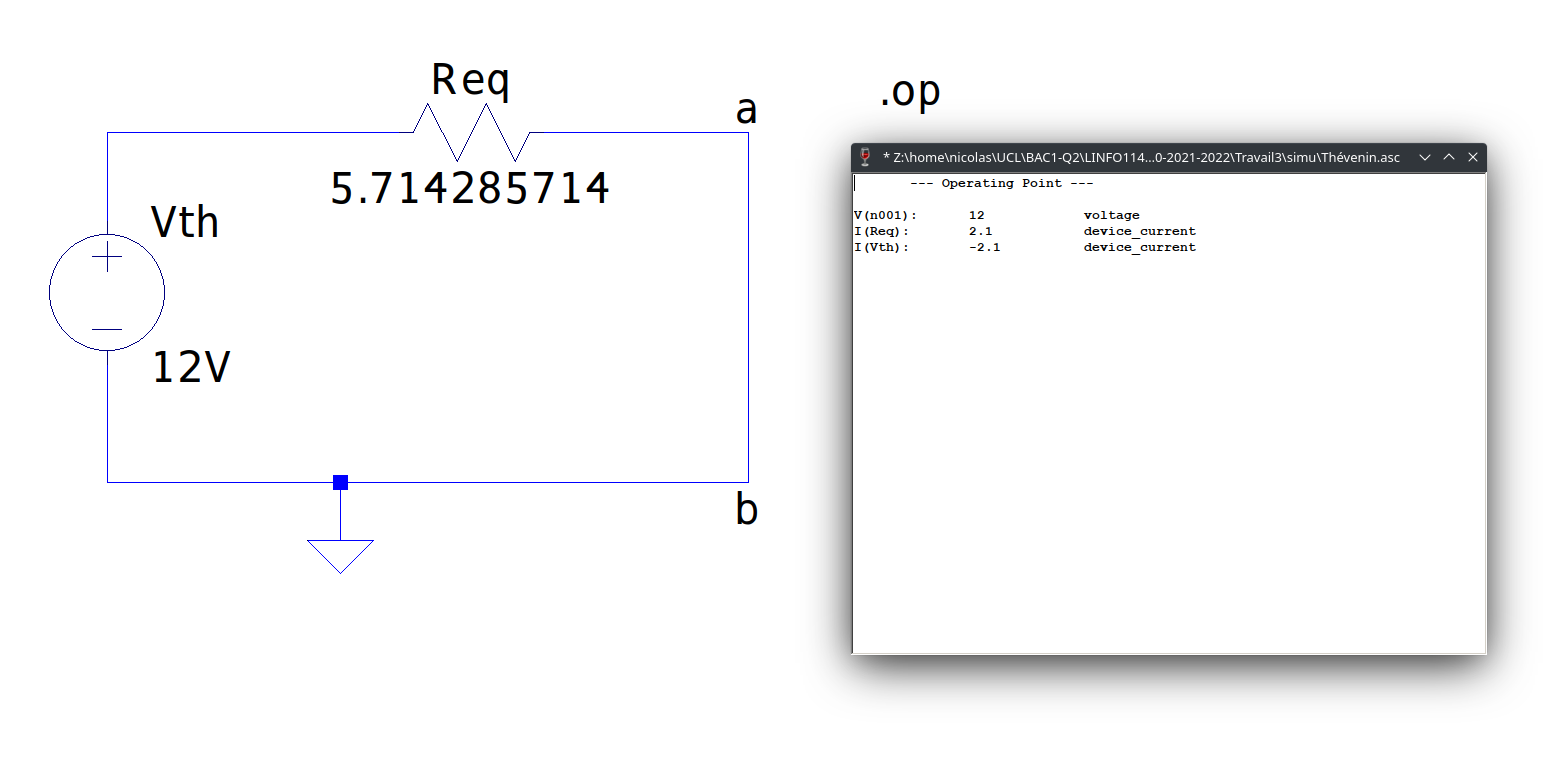
\includegraphics[width=\textwidth]{../pictures/thevenin.png}
        \caption{Équivalent de Thévenin}
    \end{figure}
    
    \begin{figure}[H]
        \centering
        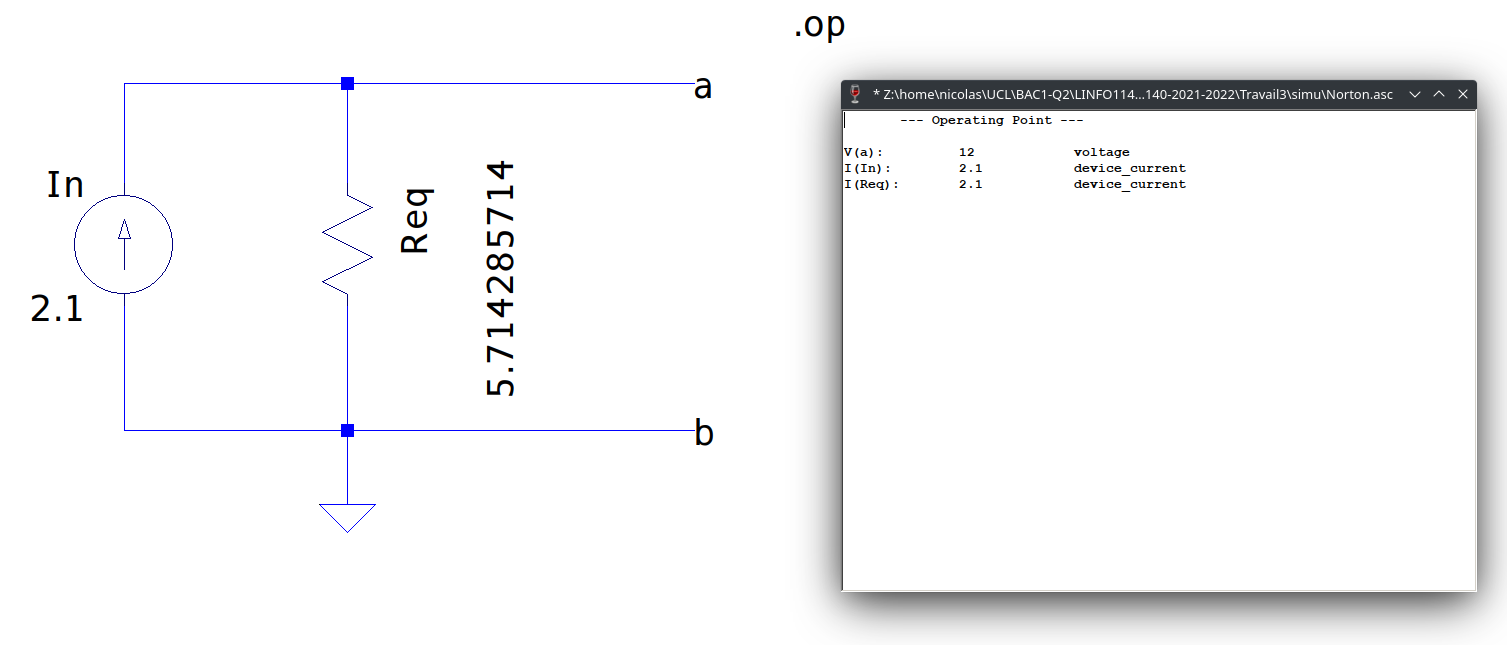
\includegraphics[width=\textwidth]{../pictures/norton.png}
        \caption{Équivalent de Norton}
    \end{figure}
    
    \subparagraph{}On peut remarquer que les valeurs fournies par $LTspice$ sont en accord avec les résultats trouvés.

\section{Simulation du circuit avec une résistance aux bornes}

    \subparagraph{}En ajoutant la résistance $R_{bornes}$ de valeur $5\;\Omega$ aux bornes on obtient les résultats suivant :
    
        \begin{figure}[H]
            \centering
            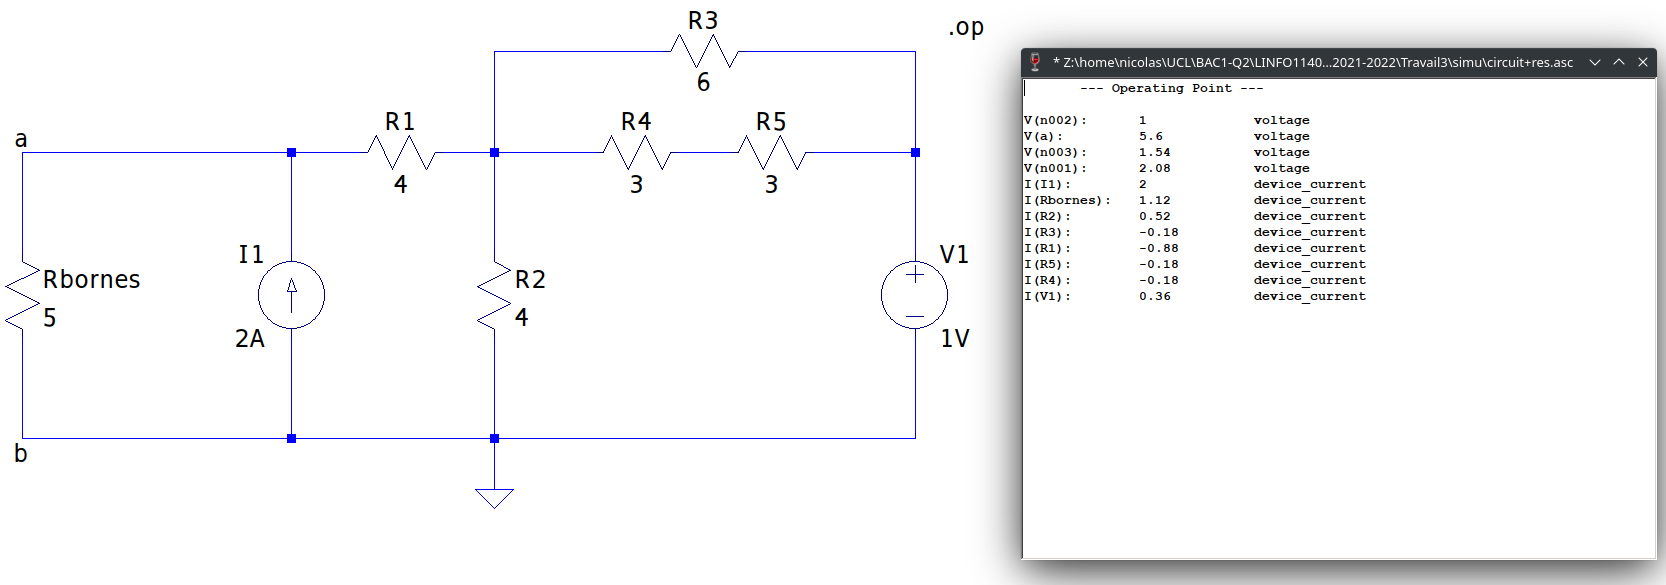
\includegraphics[width=\textwidth]{../pictures/c+r.png}
            \caption{Circuit avec la résistances aux bornes}
        \end{figure}
    
        \begin{figure}[H]
            \centering
            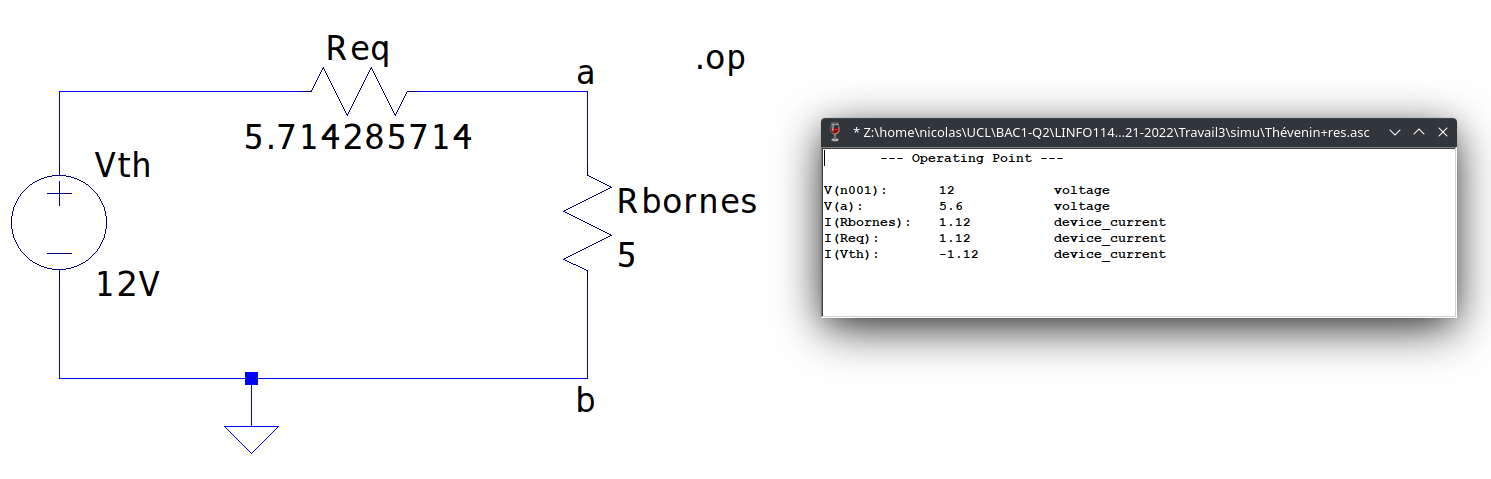
\includegraphics[width=\textwidth]{../pictures/t+r.png}
            \caption{Équivalent de Thévenin avec la résistances aux bornes}
        \end{figure}
    
        \begin{figure}[H]
            \centering
            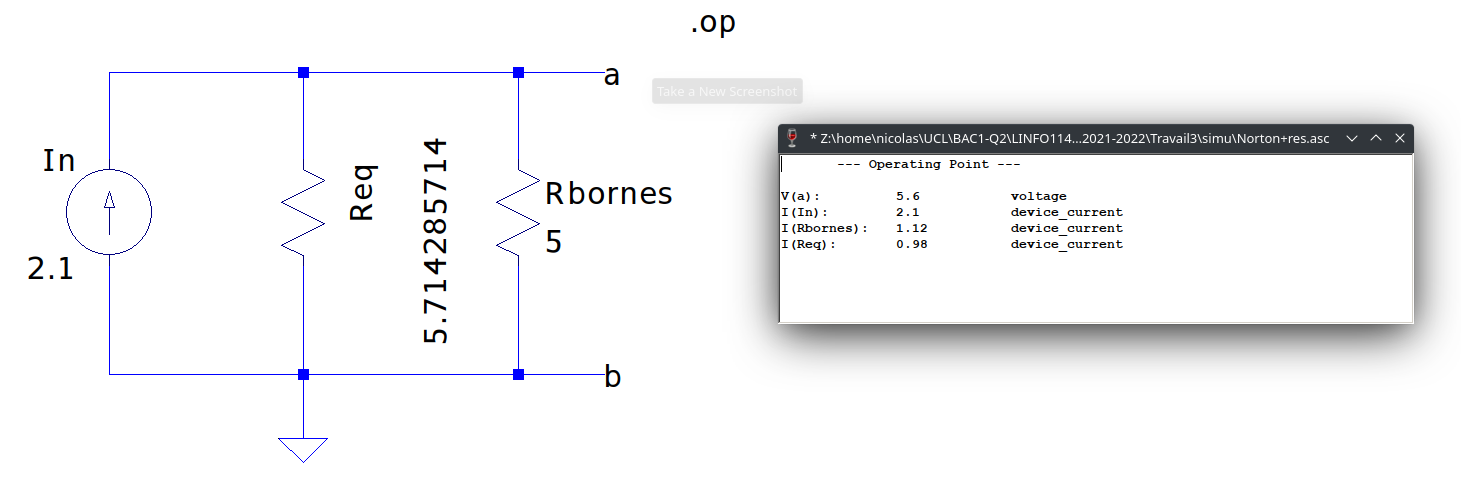
\includegraphics[width=\textwidth]{../pictures/n+r.png}
            \caption{Équivalent de Norton avec la résistances aux bornes}
        \end{figure}

\section{Conclusion}

    Pour conclure, les résultats obtenus au point \textbf{5} permettent de prouver que mes calculs sont bons vu que $V_a$ est égal à 5.6 V dans les 3 cas pour une résistance de 5 $\Omega$. Ce travail a vraiment pu me permettre de bien assimiler ce point de matière.

\end{document}

\end{document}